\newgeometry{outer=1.65cm,inner=1.65cm,top=1.75cm,bottom=1.75cm,
  marginparwidth=1.1cm,marginparsep=.2cm}
\chapter{A chave privada de um gerador}
\label{chapter:dlog-relations}
\label{page:dlog-relations-start}

\begingroup
\footnotesize
\setstretch{1.0}
\titleformat{\section}{\normalfont\large\bfseries}{\thesection}{.7em}{}
\titlespacing*{\section}{0pt}{1.1ex plus .3ex minus .2ex}{.55ex}
\titleformat{\subsection}{\normalfont\footnotesize\bfseries}{}{0pt}{}
\titlespacing*{\subsection}{0pt}{.52ex plus .15ex minus .1ex}{.18ex}
\setlength{\parskip}{.62ex plus .2ex minus .15ex}
\setlength{\abovedisplayskip}{3pt plus 2pt minus 1pt}
\setlength{\belowdisplayskip}{3pt plus 2pt minus 1pt}
\setlength{\abovedisplayshortskip}{2pt plus 1pt}
\setlength{\belowdisplayshortskip}{2pt plus 1pt}

Chamaram-lhes por vezes «chaves privadas dos geradores». A alcunha é boa,
desde que não ponha duas criaturas diferentes dentro do mesmo sobretudo. Uma
chave privada vulgar é intencional:
\[
 P=xG,
\]
e o dono deve conhecer \(x\). Uma armadilha de parâmetros é antes uma relação
que o protocolo precisava que ninguém soubesse, por exemplo
\[
 B=qA,
\]
ou, com mais bases,
\[
 a_1J_1+\cdots+a_nJ_n=\mathcal O.
\]
A segunda relação pode ser conhecida sem oferecer um quociente conveniente
entre um par escolhido: os outros termos continuam no caminho. A hipótese
certa é, pois, a \emph{vinculação por logaritmo discreto generalizado}, não
uma colecção de «três gammas secretos».

Também importa \emph{quem} sabe. Uma relação deliberadamente pública pode ser
parte do protocolo; uma relação escondida pelo criador dos parâmetros é uma
porta das traseiras; uma descoberta posterior torna a porta pública daquele
momento em diante. Esta última não extrai retroactivamente todas as chaves
ordinárias. A pessoa que queira reabrir um ponto continua muitas vezes a
precisar de uma primeira abertura.

\begin{center}
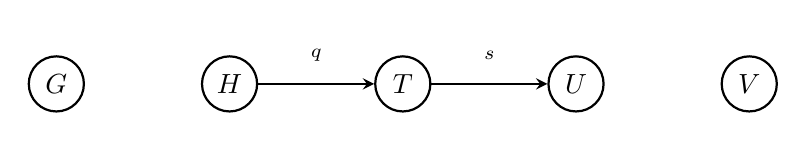
\begin{tikzpicture}[>=stealth,thick,
  every node/.style={circle,draw,minimum size=7mm,inner sep=1pt}]
 \node (G) at (0,0) {\(G\)};
 \node (H) at (2.2,0) {\(H\)};
 \node (T) at (4.4,0) {\(T\)};
 \node (U) at (6.6,0) {\(U\)};
 \node (V) at (8.8,0) {\(V\)};
 \draw[->] (H) -- node[draw=none,rectangle,above] {\scriptsize \(q\)} (T);
 \draw[->] (T) -- node[draw=none,rectangle,above] {\scriptsize \(s\)} (U);
\end{tikzpicture}

\vspace{2pt}
\(\displaystyle H\xrightarrow{q}T\xrightarrow{s}U
       \Longrightarrow U=(sq)H.\)
\end{center}

Este é o \emph{grafo de relações}. Os vértices são geradores; uma aresta
\(A\xrightarrow{q}B\) significa \(B=qA\). Como os escalares não nulos têm
inverso, o caminho pode ser percorrido para trás, e os rótulos multiplicam-se.
Cada componente ligada entrega todos os logaritmos aos pares \emph{dentro}
dela. No desenho, porém, \(G\) e \(V\) continuam ilhas: conhecer a aresta
\(H-T\) não revela \(\log_GH\). Uma relação de aridade superior é uma
hiper-aresta e não cabe inteiramente neste desenho.

Convém ainda separar as consequências. Neste capítulo usaremos cinco carimbos:
\emph{exploração algébrica directa}; \emph{exploração provável que exige
composição}; \emph{falha só de privacidade}; \emph{hipótese de segurança
invalidada sem exploração concreta demonstrada}; e \emph{relação inofensiva
ou deliberadamente conhecida}. Roubo, gasto duplo, pertença falsa, prova de
intervalo falsa e inflação não são sinónimos. Uma campainha partida não abre
necessariamente o cofre; às vezes limita-se, com notável profissionalismo, a
deixar de tocar.

As equações seguintes foram confrontadas com os geradores do Monero e com a
SAL corrente nas revisões fixadas nas notas do capítulo anterior
\cite{monero-source-v16,monero-oxide-fcmp-source}, e com a especificação e a
análise de composição FCMP++ \cite{fcmp-plus-plus-paper,fcmp-composition-review}.

\clearpage
\section{O antecedente: montante; o recém-chegado: saída}

\subsection*{Se \(H=\gamma G\)}

Um compromisso de montante é
\[
 C=aG+bH=(a+b\gamma)G.
\]
Quem conhece uma abertura \((a,b)\) e a armadilha escolhe \(b'\) e calcula
\[
 \boxed{\quad b\longmapsto b',\qquad
        a'=a+(b-b')\gamma\quad}
\]
porque \(a'G+b'H=aG+bH\). Perdeu-se a vinculação do montante, não a sua
ocultação. Um estranho que só vê \(C\) ainda precisa de
\(\log_G C=a+b\gamma\); o dono de uma saída, pelo contrário, já conhece
\((a,b)\). Pode reabri-la como uma entrada maior, criar novas saídas com
montantes honestamente dentro de 64 bits, produzir as provas de intervalo e
fechar a equação de balanço com a máscara \(a'\). A autorização continua a
ser da sua moeda; o valor inventado é que não era dela.

\textbf{Conclusão --- exploração algébrica directa:} \(G-H\) destrói a
vinculação de compromissos existentes cujas aberturas o atacante conhece e,
composta com o balanço e as provas de intervalo normais, permite inflação
oculta. Não dá ao portador de \(\gamma\) a chave de gasto de uma saída alheia.
O capítulo \ref{chapter:transactions} deriva esta transacção passo a passo.

\subsection*{Se \(T=\tau G\)}

A chave de saída compatível com formatos antigos e futuros é
\[
 O=xG+yT=(x+y\tau)G.
\]
De uma abertura sai uma família inteira:
\[
 y\longmapsto y',\qquad x'=x+(y-y')\tau,\qquad
 O=x'G+y'T.
\]
Mas um estranho diante de um \(O\) arbitrário ainda não conhece
\(k=\log_GO=x+y\tau\). Portanto \(\tau\), sozinho, não rouba essa saída. O
que desaparece é o significado independente das duas coordenadas: migrações
e formatos futuros não podem atribuir poderes diferentes a \(x\) e \(y\), e
uma prova SAL de «conheço \(x,y\)» deixa de provar a abertura pretendida.

Há uma consequência concreta para o próprio dono. Numa saída histórica
\(O=xG\), a árvore conserva também \(I=\mathcal H_p(O)\), e a SAL publica
\(L=xI\). Com \(\tau\), o dono escolhe aberturas alternativas \(x'\) do mesmo
\(O\) e obtém marcadores \(L'=x'I\) diferentes. A autorização não passou para
um estranho; a detecção do segundo gasto deixou de reconhecer o primeiro.

\textbf{Conclusão --- exploração algébrica directa:} \(G-T\) permite ao dono
de uma saída afectada quebrar a ligação SAL e tentar o gasto duplo. O roubo
por um observador não foi demonstrado; falta-lhe uma abertura de \(O\).

\subsection*{As três pontes de \(H\)}

Se \(H=qT\), \(H=qU\) ou \(H=qV\), a aresta liga a família de montantes à
família FCMP++, mas \(H\) e a outra base não aparecem juntas num compromisso
de montante com coeficientes variáveis. A aresta isolada não dá
\(\log_GH\), não reabre \(C=aG+bH\) e não é inflação. Se outra aresta ligar
essa componente a \(G\), o caminho compõe-se: por exemplo,
\(H=qU,\ U=uG\) dá \(H=(qu)G\), e regressamos ao ataque de \(\gamma\).

\textbf{Conclusão --- hipótese invalidada sem exploração concreta
demonstrada:} cada uma de \(H-T,H-U,H-V\), sozinha. Com um caminho adicional
até \(G\), a inflação passa a ser a exploração directa anterior.

\subsection*{A base que muda com a saída}

\(\mathcal H_p(O)\) não é um sexto parâmetro estático. Se, para uma saída
histórica, alguém descobre
\[
 \mathcal H_p(O)=\eta_OG,\qquad O=xG,\qquad
 L=x\mathcal H_p(O),
\]
então
\[
 \boxed{L=\eta_OO.}
\]
O marcador da saída torna-se calculável a partir de dados públicos. Conhecer
\(\eta_O\) para uma saída permite reconhecê-la quando \(L\) aparece; conhecer
as relações para todas permite varrer a cadeia. Não revela \(x\), não assina
uma transacção e não faz \(L\) deixar de repetir.

\textbf{Conclusão --- falha só de privacidade:} identificação retroactiva da
saída gasta; sem roubo, sem quebra da autorização e sem inflação demonstrada.

\clearpage
\section{SAL: quatro bases, um produto e três maneiras de cortar o fio}
\scriptsize

O código corrente não se limita a \(\widetilde I\) e \(R_{\rm fcmp}\). Para
uma abertura \(O=xG+yT\), escreve, com \(z=xr_i\),
\begin{align*}
 \widetilde I&=I+r_iU,&
 R_{\rm fcmp}&=r_iV+r_jT,\\
 P&=xG+r_iV+zU+r_pT,& z&=xr_i,\\
 P-\widetilde O-R_{\rm fcmp}&=zU+r_p''T,&
 L&=x\widetilde I-zU.
\end{align*}
A prova de produto prende \(z=xr_i\) dentro de \(P\); três provas de
representação prendem \(x\) a \(\widetilde O\), \(z\) à terceira linha e
\((x,z)\) a \(L\). A pertença FCMP prende o seu \(r_i\) simultaneamente a
\(\widetilde I\) e \(R_{\rm fcmp}\). É uma costura: cada ponto público faz
duas peças dizerem «usei o mesmo escalar».

\subsection*{\(U=qT\): muda o coeficiente de \(U\)}

Para quaisquer \(a,b,\Delta\),
\[
 aU+bT=(a+\Delta)U+(b-q\Delta)T.
\]
Assim, \(zU+r_p''T\) aceita um \(z_{\rm lig}\) diferente do
\(z_{\rm prod}=xr_i\) provado dentro de \(P\), ajustando a máscara em \(T\).
A última equação publica então
\[
 L=x\widetilde I-z_{\rm lig}U,
\]
que o dono pode variar entre gastos da mesma folha. A armadilha não muda
\(r_i\) em \(\widetilde I=I+r_iU\); muda a interpretação do coeficiente de
\(U\) onde \(T\) lhe serve de cortina.

\textbf{Conclusão --- exploração algébrica directa:} falha de ligação SAL e
gasto duplo pelo dono; não roubo de uma saída arbitrária.

\subsection*{\(V=qT\): \(R_{\rm fcmp}\) já não se compromete com \(r_i\)}

Agora
\[
 r_iV+r_jT=(r_i+\Delta)V+(r_j-q\Delta)T.
\]
A prova FCMP pode usar o \(r_i\) que abre \(\widetilde I\), enquanto a SAL
usa \(r_i'=r_i+\Delta\) no produto \(z'=xr_i'\); o mesmo ponto
\(R_{\rm fcmp}\) conta as duas histórias. O termo extra em \(V\) é absorvido
pela máscara em \(T\) de \(P\). Resulta
\(L=x\widetilde I-xr_i'U\), variável com \(\Delta\).

\textbf{Conclusão --- exploração algébrica directa:} perdeu-se exactamente
o compromisso a \(r_i\) que compunha pertença e SAL; o dono pode produzir
marcadores diferentes.

\subsection*{\(V=qU\): produto certo, ligação errada}

No ponto \(P\),
\[
 r_iV+zU=(r_i+\Delta)V+(z-q\Delta)U.
\]
Mais explicitamente, deixe a pertença usar \(r\), a prova de produto usar
\(r'\) e \(z'=xr'\). Depois de subtrair \(R_{\rm fcmp}\), a prova de
representação lê
\[
 z_{\rm lig}=xr'+q(r'-r),
\]
logo
\[
 L=xI+(x+q)(r-r')U.
\]
Escolher \(r'\) muda \(L\), salvo o caso degenerado \(x=-q\).

\textbf{Conclusão --- exploração algébrica directa:} novamente gasto duplo
por quebra da ligação; ainda exige conhecer uma abertura autorizada da saída.

\subsection*{\(U=qG\) e \(V=qG\): uma fenda que as outras linhas tapam}

Se \(U=qG\), \(xG+zU\) admite
\((x,z)\mapsto(x-q\Delta,z+\Delta)\). Se \(V=qG\), \(xG+r_iV\)
admite o mesmo deslocamento em \((x,r_i)\). A vinculação interna de \(P\)
desaparece. Isoladamente, porém, \(\widetilde O=xG+yT\) fixa \(x\),
\(R_{\rm fcmp}=r_iV+r_jT\) fixa \(r_i\), e a equação em \(U,T\) fixa \(z\),
sob as relações restantes desconhecidas. Não obtivemos uma transacção falsa.

\textbf{Conclusão --- hipótese de segurança invalidada sem exploração
concreta demonstrada:} \(G-U\) e \(G-V\) isoladas; outra aresta que permita
absorver uma destas diferenças pode completar o ataque.

\subsection*{A forma que contém todos os pares}

Se for conhecida
\[
 aG+bT+cU+dV=\mathcal O,
\]
então qualquer compromisso multibase
\[
 M=xG+pT+zU+rV
\]
conserva o ponto sob a seta
\[
 (x,p,z,r)\longmapsto
 (x,p,z,r)+\lambda(a,b,c,d).
\]
Isto é perda directa de vinculação do vector-testemunho. A consequência final
depende dos coeficientes que as equações externas voltam a fixar; os três
ataques acima mostram relações cujo suporte corta a costura certa. Uma relação
de aridade superior não deve ser promovida automaticamente a inflação, nem
rebaixada por não oferecer \(\log_GT\) numa bandeja.

\begin{landscape}
\section{As dez arestas, sem adivinhação}

\scriptsize
\setlength{\tabcolsep}{3pt}
\renewcommand{\arraystretch}{1.05}
\begin{center}
\begin{tabular}{|p{.72in}|p{1.80in}|p{2.48in}|p{1.38in}|p{1.36in}|}
\hline
\textbf{Relação conhecida} & \textbf{Equação pública e abertura alternativa}
& \textbf{Quem a explora; saídas já existentes} & \textbf{Resultado isolado}
& \textbf{Outra armadilha?}\\ \hline
\(H=\gamma G\) & \(C=aG+bH\);
\(b'\), \(a'=a+(b-b')\gamma\). & Quem conhece a abertura; sim, compromissos
próprios antigos continuam reabríveis. & Montante não vinculante; inflação
oculta pela transacção normal. & Não; requer apenas autorização de uma entrada
e as provas normais.\\ \hline
\(T=\tau G\) & \(O=xG+yT\);
\(y'\), \(x'=x+(y-y')\tau\). & Só quem conhece uma abertura; sim, saídas
históricas próprias migradas. & Autorização ambígua; \(L\) variável, gasto
duplo. Não rouba \(O\) arbitrário. & Não para o dono; ao estranho falta
\(\log_GO\).\\ \hline
\(U=qG\) & \(P\) contém \(xG+zU\);
\((x,z)\mapsto(x-q\Delta,z+\Delta)\). & Provador com uma abertura; pontos
existentes têm duas descrições locais. & Vinculação de \(P\) perdida, mas
\(\widetilde O\) e a equação \(U,T\) bloqueiam a falsificação completa. & Sim,
uma relação que absorva a diferença externa.\\ \hline
\(V=qG\) & \(P\) contém \(xG+r_iV\);
\((x,r_i)\mapsto(x-q\Delta,r_i+\Delta)\). & Provador com uma abertura; a
descrição local de \(P\) muda. & Redução SAL invalidada; \(\widetilde O\) e
\(R_{\rm fcmp}\) fixam os coeficientes em isolamento. & Sim.\\ \hline
\(H=qT\) & \(C\) usa \(G,H\); saída/SAL usa \(G,T\). Não há compromisso
variável comum a \(H,T\). & Ninguém obtém nova abertura só com a aresta; saídas
existentes inalteradas. & Famílias ligadas; sem inflação ou roubo demonstrado.
& Sim: caminho de \(T\) até \(G\) dá \(\log_GH\).\\ \hline
\(H=qU\) & \(C\) usa \(G,H\); SAL usa \(G,T,U,V\). Aresta não basta para
deslocar \(a,b\). & Idem; sem efeito concreto retroactivo isolado. & Hipótese
global invalidada, sem exploração concreta. & Sim: caminho de \(U\) até
\(G\).\\ \hline
\(H=qV\) & Mesma separação: \(H\) não aparece nas equações SAL. & Idem. & Sem
exploração concreta demonstrada. & Sim: caminho de \(V\) até \(G\).\\ \hline
\(U=qT\) & \(zU+pT=(z+\Delta)U+(p-q\Delta)T\). & Dono/provador autorizado;
sim, pode gastar a mesma folha existente com outro \(L\). & Coeficiente \(z\)
da ligação difere do produto; gasto duplo. & Não.\\ \hline
\(V=qT\) & \(R=r_iV+r_jT=(r_i+\Delta)V+(r_j-q\Delta)T\). & Dono/provador;
sim, FCMP e SAL podem abrir o mesmo \(R\) com \(r_i\) diferentes. & Compromisso
a \(r_i\) perdido; \(L\) variável, gasto duplo. & Não.\\ \hline
\(V=qU\) & \(r_iV+zU=(r_i+\Delta)V+(z-q\Delta)U\). & Dono/provador; sim,
uma folha autorizada basta. & Produto e ligação recebem aberturas distintas;
gasto duplo. & Não.\\ \hline
\end{tabular}
\end{center}

\footnotesize
«Existentes» não quer dizer que um estranho possa escolher a moeda de Alice.
Quer dizer que, depois da descoberta, o titular que ainda conserva a abertura
consegue aplicá-la ao ponto já publicado. O criador malicioso dos parâmetros
teve essa possibilidade desde o princípio; uma descoberta pública dá-a a
todos os titulares e simultaneamente dá aos verificadores a oportunidade de
parar, actualizar regras ou rejeitar a família comprometida. Provas antigas
não se apagam por cortesia.
\end{landscape}

\footnotesize
\section{Bulletproofs: quando o intervalo deixa de ser uma cerca}

As bases indexadas das Bulletproofs e Bulletproof+ formam compromissos do
género
\[
 Q=\rho H+\langle\boldsymbol a,\boldsymbol G\rangle
       +\langle\boldsymbol b,\boldsymbol H\rangle.
\]
Na notação concreta do Monero, \(G\) desempenha também o papel de base de
algumas máscaras internas e \(H\) leva o montante; a troca de nomes não muda
o argumento. Suponhamos conhecida uma relação
\[
 \rho_0H+\langle\boldsymbol u,\boldsymbol G\rangle
       +\langle\boldsymbol v,\boldsymbol H\rangle=\mathcal O.
\]
Então, sem mudar \(Q\), existe a seta
\[
 (\rho,\boldsymbol a,\boldsymbol b)\longmapsto
 (\rho,\boldsymbol a,\boldsymbol b)
       +\lambda(\rho_0,\boldsymbol u,\boldsymbol v).
\]
Uma abertura vectorial já não fixa os bits, os vectores de produtos ou as
máscaras que as equações de produto interno pretendiam coser. É a mesma
doença de Pedersen, agora com muitos sintomas \cite{Bulletproofs_paper}.

Isto não autoriza a frase «qualquer relação vectorial fabrica dinheiro». Uma
relação pode cair numa direcção que não altera a coordenada constrangida, ou
invalidar apenas a redução sem oferecer uma transcrição falsa. Se a direcção
permite trocar um vector inválido por uma abertura que satisfaz as equações da
prova, porém, a solidez de intervalo desaparece: um compromisso fora de
\([0,2^{64}-1]\) pode receber uma prova aceite.

\begin{center}
\begin{tikzpicture}[>=stealth,node distance=8mm,
 box/.style={draw,rounded corners,align=center,text width=3.0cm,
 minimum height=9mm,inner sep=3pt}]
 \node[box,fill=yellow!18] (rel) {relação vectorial\\utilizável};
 \node[box,fill=orange!18,right=of rel,xshift=5mm] (proof)
 {abertura alternativa\\prova de intervalo falsa};
 \node[box,fill=red!12,right=of proof,xshift=5mm] (bal)
 {balanço modular\\saídas válidas};
 \draw[->] (rel) -- (proof);
 \draw[->] (proof) -- (bal);
 \node[draw=none,below=2mm of bal] {\(\Downarrow\) inflação};
\end{tikzpicture}
\end{center}

O compromisso não vinculante \(G-H\) dá a primeira rota directa. Uma prova de
intervalo falsa dá outra: permite que a aritmética módulo \(l\) esconda um
valor negativo ou transbordado, enquanto as saídas recebidas parecem montantes
canónicos. É uma \emph{exploração provável que exige composição} com uma
relação que atinja os testemunhos certos, o balanço da transacção e a criação
de novos compromissos. Não rouba por si só uma chave de saída e não torna
falsas, retroactivamente, todas as provas antigas.

\subsection*{O controlo negativo}

As tabelas
\[
 J, 2J, 4J,\ldots,2^{n-1}J
\]
usadas pelo dispositivo de logaritmo discreto têm relações públicas por
desenho: os dígitos recompõem um múltiplo. Também \(P=xG\), um nonce \(R=rH\)
e qualquer ponto construído com testemunho conhecido são declarações, não
falhas de parâmetros. A solidez vem da prova de conhecimento e das restantes
restrições, não de fingir que \(2J\) nasceu sem família. \textbf{Conclusão ---
relação inofensiva ou deliberadamente conhecida.}

\clearpage
\section{Curve Trees, Selene e Helios: uma raiz não é uma escritura}

Cada curva tem a sua própria família
\[
 g, h, \boldsymbol g, \boldsymbol h, J_{\rm init}.
\]
Selene e Helios são grupos distintos: não há um caminho de arestas que
atravesse de uma curva para a outra. Em cada uma, os compromissos da prova têm
a forma
\[
 Q=rh+\langle\boldsymbol a,\boldsymbol g\rangle
       +\langle\boldsymbol b,\boldsymbol h\rangle,
\]
e um nó que compromete os filhos tem a forma
\[
 N=J_{\rm init}+\sum_i v_iJ_i.
\]
As famílias são derivadas de rótulos separados e sem cerimónia confiada na
implementação consultada; «transparente» significa que todos reproduzem os
pontos, não que uma relação linear conhecida fosse aceitável
\cite{curve-trees,generalized-bulletproofs-review}.

Uma relação entre \(h,\boldsymbol g,\boldsymbol h\) dá aberturas alternativas
dos compromissos da prova, como na secção anterior. Uma relação
\(\sum_i d_iJ_i=\mathcal O\) dá uma colisão explícita entre vectores de
filhos:
\[
 (v_0,\ldots,v_m)\longmapsto
 (v_0,\ldots,v_m)+\lambda(d_0,\ldots,d_m),
 \qquad N\ \hbox{inalterado}.
\]
Se essa colisão troca um filho honesto por outro compromisso, pode fabricar
uma passagem falsa numa camada e propagá-la honestamente até à raiz. Relações
que envolvem \(g\) ou as bases vectoriais podem, em vez disso, falsificar as
restrições de selecção e re-randomização. O resultado possível é uma prova de
pertença de uma saída que nunca esteve na árvore.

\(J_{\rm init}\) merece uma vírgula. Se o seu coeficiente é sempre exactamente
um, ele cancela ao comparar dois nós bem formados; conhecer apenas
\(J_{\rm init}=qJ_0\) não produz automaticamente dois vectores de filhos com o
mesmo nó. A relação torna-se utilizável se o inicializador puder ser absorvido
por uma máscara da prova, se colidir uma codificação inicializada com uma soma
crua, ou se vier acompanhada de uma relação entre os \(J_i\). Sem essa
composição, temos hipótese invalidada, não uma árvore falsa demonstrada.

No topo há ainda a prova Schnorr da abertura da raiz. Se
\[
 X=\widehat{\mathcal R}_{\rm tree}-\mathcal R_{\rm tree}=\rho h,
\]
o verificador exige
\[
 R_{\rm sig}+cX=sh.
\]
Uma armadilha que permita converter uma diferença de \emph{conteúdo} falsa
num múltiplo conhecido de \(h\) faz esta equação aceitar a raiz comprometida.
Saber apenas um caminho verdadeiro não faz isso: permite provar pertença do
membro verdadeiro, que é precisamente o serviço comprado.

\begin{center}
\begin{tikzpicture}[>=stealth,node distance=7mm,
 box/.style={draw,rounded corners,align=center,text width=2.55cm,
 minimum height=9mm,inner sep=3pt}]
 \node[box,fill=yellow!17] (trap) {relação utilizável\\numa das curvas};
 \node[box,fill=orange!15,right=of trap,xshift=4mm] (path)
 {colisão ou restrição falsa\\caminho FCMP falso};
 \node[box,fill=blue!12,right=of path,xshift=4mm] (sal)
 {saída fabricada, mas própria\\SAL válida};
 \draw[->] (trap) -- (path);
 \draw[->] (path) -- (sal);
 \node[draw=none,below=2mm of sal] {\(\Downarrow\) entrada inexistente \(\Rightarrow\) inflação};
\end{tikzpicture}
\end{center}

Pertença falsa, sozinha, não é autorização. Provar que a saída de Alice está
na floresta não revela \(x\) e não produz a SAL. Para chegar à inflação, o
atacante fabrica uma tupla que ele próprio sabe abrir, atribui-lhe um
compromisso de montante, usa a armadilha para provar um caminho inexistente e
produz uma SAL válida. A entrada sem antepassado financia saídas novas. É uma
\emph{exploração provável que exige composição}: armadilha utilizável de
Selene \emph{ou} Helios, pertença falsa concreta, saída fabricada possuída e
balanço válido. Roubo de uma saída alheia não resulta da pertença falsa.

Esta conclusão vale separadamente nas duas curvas. Uma colisão utilizável numa
camada Selene pode bastar sem uma armadilha Helios, e vice-versa; uma relação
que só reabre um compromisso auxiliar mas não altera uma restrição relevante
pode ficar no nível «solidez assumida, exploração não demonstrada».

\begin{landscape}
\section{Matriz de consequências}

\tiny
\setlength{\tabcolsep}{1.8pt}
\renewcommand{\arraystretch}{.98}
\begin{center}
\begin{tabular}{|p{.62in}|p{.67in}|p{.84in}|p{.43in}|p{.43in}|p{.52in}|p{.52in}|p{.62in}|p{.52in}|p{.82in}|p{.78in}|}
\hline
\textbf{Família} & \textbf{Armadilha conhecida} & \textbf{Vinculação perdida onde}
& \textbf{\shortstack{Privaci-\\dade?}} & \textbf{Roubo?} & \textbf{Pertença falsa?}
& \textbf{Intervalo falso?} & \textbf{Detecção gasto duplo?}
& \textbf{Inflação?} & \textbf{Hipóteses adicionais} & \textbf{Confiança / evidência}\\ \hline
\(G,H\) & \(H=\gamma G\) & compromisso de montante & no & no & no & no & no & yes
& abertura e transacção normal & alta: álgebra e código RingCT\\ \hline
\(G,T\) & \(T=\tau G\) & abertura \(x,y\) da saída & no & no & no & no & yes & conditional
& abertura própria; segundo gasto & alta: álgebra SAL/código\\ \hline
\(G,U\) & \(U=qG\) & \(x,z\) dentro de \(P\) & no & no & no & no & conditional & conditional
& outra relação que vença \(O,P'\) & média: álgebra; exploração não demonstrada\\ \hline
\(G,V\) & \(V=qG\) & \(x,r_i\) dentro de \(P\) & no & no & no & no & conditional & conditional
& outra relação que vença \(O,R\) & média: álgebra; exploração não demonstrada\\ \hline
\(H,T\) & \(H=qT\) & nenhuma equação isolada & no & no & no & no & no & conditional
& caminho \(T\leadsto G\) & alta: grafo e equações separadas\\ \hline
\(H,U\) & \(H=qU\) & nenhuma equação isolada & no & no & no & no & no & conditional
& caminho \(U\leadsto G\) & alta: grafo e equações separadas\\ \hline
\(H,V\) & \(H=qV\) & nenhuma equação isolada & no & no & no & no & no & conditional
& caminho \(V\leadsto G\) & alta: grafo e equações separadas\\ \hline
\(T,U\) & \(U=qT\) & \(zU+rT\) & no & no & no & no & yes & conditional
& abertura própria; segundo gasto & alta: deslocação SAL explícita\\ \hline
\(T,V\) & \(V=qT\) & \(R_{\rm fcmp}\) em \(r_i\) & no & no & no & no & yes & conditional
& abertura própria; segundo gasto & alta: deslocação SAL explícita\\ \hline
\(U,V\) & \(V=qU\) & \(r_iV+zU\) & no & no & no & no & yes & conditional
& abertura própria; segundo gasto & alta: deslocação SAL explícita\\ \hline
\(G,T,U,V\) & \(aG+bT+cU+dV=0\) & compromisso multibase & condi\-tional & not demonstrated & condi\-tional & no & condi\-tional & condi\-tional
& suporte deve vencer equações externas & média: vinculação certa; efeito depende do suporte\\ \hline
\(\mathcal H_p(O)\) & \(\mathcal H_p(O)=\eta_OG\) & bases da DLEQ tornam-se relacionadas & yes & no & no & no & no & no
& relação para a saída observada & alta: \(L=\eta_OO\)\\ \hline
BP/BP+ & relação em \(H,\boldsymbol G,\boldsymbol H\) & compromisso vectorial & no & no & no & conditional & no & conditional
& direcção altera testemunho; balanço & média: abertura explícita; falsificação depende da relação\\ \hline
Selene & relação em \(g,h,\boldsymbol g,\boldsymbol h,J_{\rm init}\) & nó ou compromisso da prova & no & no & conditional & no & no & conditional
& colisão/restrição útil; saída própria e SAL & média: Curve Trees e composição\\ \hline
Helios & relação em \(g,h,\boldsymbol g,\boldsymbol h,J_{\rm init}\) & nó ou compromisso da prova & no & no & conditional & no & no & conditional
& colisão/restrição útil; saída própria e SAL & média: Curve Trees e composição\\ \hline
Controlo & \(J,2J,\ldots;\ P=xG;\ R=rH\) & nenhuma & no & no & no & no & no & no
& prova de conhecimento normal & alta: relação deliberada\\ \hline
\end{tabular}
\end{center}

\scriptsize
O único «yes» directo na coluna de inflação é \(G-H\). As arestas SAL
assinaladas quebram directamente a ligação, mas a inflação vem
condicionalmente de um segundo gasto. Bulletproofs e Curve Trees exigem uma
relação que atinja a restrição certa e a composição indicada. \(\eta_O\) é
privacidade sem autorização; «hipótese invalidada» continua a merecer
reparação mesmo sem assalto concreto demonstrado.

\label{page:dlog-relations-end}
\end{landscape}
\endgroup
\restoregeometry
